\documentclass[t, screen, aspectratio=43]{beamer}
\usepackage[T1]{fontenc}
\usepackage[utf8]{inputenc}
\usepackage{epsf}
\usepackage{graphicx}
\usepackage{geometry}
\usepackage{tabularx}
\usepackage[table]{colortbl}
\usepackage{xcolor}
\usepackage{soul}
\usepackage[normalem]{ulem}
\usepackage{tikz}
\usepackage{subcaption}
\usepackage{hyperref}
\usepackage{color,soul}
\usepackage{skak}
% Use the NTNU-temaet for beamer 
% \usetheme[style=ntnu|simple|vertical|horizontal, 
%     language=bm|nn|en, 
%     smalltitle, 
%     city=all|trondheim|alesund|gjovik]{ntnu2017}
\usetheme[style=helvet,language=en]{ntnu2017}

\usepackage[english]{babel}
\usepackage[style=numeric,backend=biber,natbib=false,sorting=none]{biblatex}

\title[Short title]{Ultra low power integer-N ADPLL}
\subtitle{Master's thesis project - meeting 7}
\author[C Nielsen]{Cole Nielsen}
\institute[NTNU]{Department of Electronic Systems, NTNU}
\date{28 February 2020  (calendar week 9)}
%\date{} % To have an empty date

\addbibresource{example.bib} % Add bibliography database

% Set the reference style to numeric.
% See here: http://tex.stackexchange.com/questions/68080/beamer-bibliography-icon
\setbeamertemplate{bibliography item}[text] 

% Set bibliography fonts to a small size.
\renewcommand*{\bibfont}{\footnotesize}

\usepackage{tikz}
\usepackage{enumitem}
\newcommand*\mycirc[1]{%
\begin{tikzpicture}[baseline=(C.base)]
	\node[draw,circle,inner sep=1pt,minimum size=3ex](C){#1};
\end{tikzpicture}}


\begin{document}

\begin{frame}
	\titlepage%
\end{frame}

% Alternatively, special title page command to get a different background
% \ntnutitlepage

% #############################################################################
% This week
% #############################################################################

\begin{frame}
	\frametitle{Overview}
	\begin{block}{For this week...}
		\begin{enumerate}[itemsep=4pt,label=\protect\mycirc{\arabic*}]
			\scriptsize
			\item PLL floorplan
			\item Loop filter V2
			\begin{itemize}[itemsep=4pt,label=---]
				\item Area/pin location aligned with floor plan.
				\item Simplified DSP operation.
				\item Changeable filter coefficients.
			\end{itemize}
			\item Spur estimate.
		\end{enumerate} 
	\end{block}	
\end{frame}


% #############################################################################
% This week
% #############################################################################


% #############################################################################
% Physical limits
% #############################################################################


\begin{frame}
	\frametitle{PLL Floorplan}
	\begin{block}{Loop filter}
		\begin{minipage}{6cm}
			\vspace{1em}
			\tiny

			% \vspace{100em}
			\begin{itemize}[itemsep=4pt,label=\protect---]
				\item Full PLL floorplan necessary to make reasonable placement of pins and to constrain size of loop filter.
				\item {\color{red}\textbf{Total area = 0.0064 mm$^2$}} (80 $\mu$m x 80 $\mu$m )
				\begin{itemize}[itemsep=4pt,label=\protect$\bullet$]
						\item \textbf{Active area = 0.00515 mm$^2$} (minus DECAP)
					\end{itemize}
				\item Loop filter architecture simplified to reduce area into 30 $\mu$m x 50 $\mu$m.
				\item 10b CDAC utilizing minimum 1$\mu$m x 1$\mu$m APMOM caps.
					\begin{itemize}[itemsep=4pt,label=\protect$\bullet$]
						\item Between 1.96-4.72 fF per unit cap (2-4.8 pF total), depending how many metal layers used.
						\item Depends on arangement, however should fit in either 25 $\mu$m x 50 $\mu$m or perhaps 30 $\mu$m x 50 $\mu$m.
					\end{itemize}
				\item Include dedicated decap for analog to help with noise?? 25 $\mu$m x 50 $\mu$m will yield ca. 30 pF.
				\item Seperate power for analog/digital
					\begin{itemize}[itemsep=4pt,label=\protect$\bullet$]
						\item Possibly 0.5 for digital and 0.8 for analog? Higher supply is better for supply rejection with VCO...
					\end{itemize}
			\end{itemize}

			% \vspace{-3em}
		\end{minipage}%
		% \hspace{-0.5cm}
		\begin{minipage}{6cm}
			\begin{figure}[htb!]
			        \centering
			        \includegraphics[width=1\textwidth, angle=0]{pll_floorplan}
			    % \caption{Approximate model for ring oscillator inverter delay cell.}
			\end{figure}
		\end{minipage}%

	\end{block}	
\end{frame}


\begin{frame}
	\frametitle{Renewed area comparison.}
	\begin{block}{5nm FinFET state of art}
	\begin{minipage}{5cm}
		\center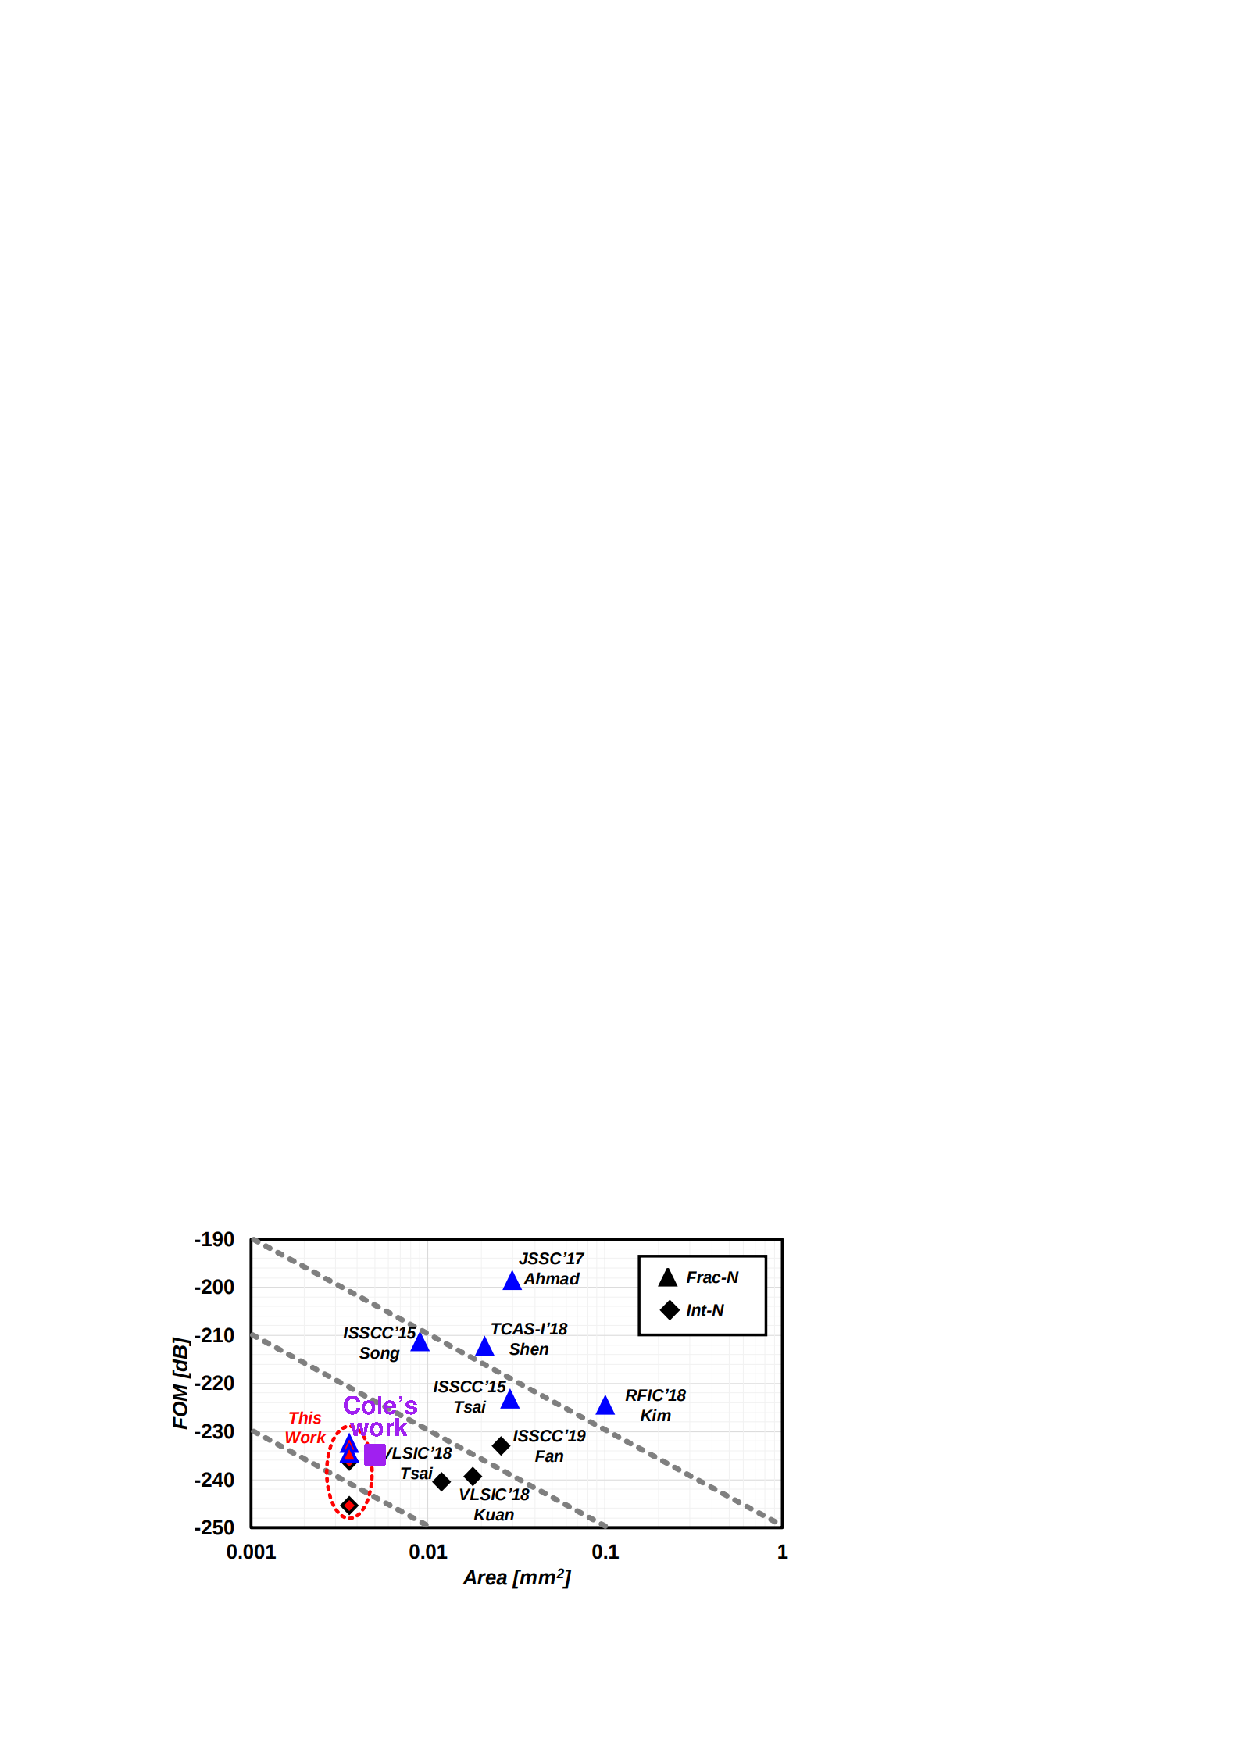
\includegraphics[width=1\textwidth, angle=0]{fom_jitter_5nm.pdf}
	\end{minipage}
	\begin{minipage}{6cm}
		\tiny
		\begin{itemize}[itemsep=4pt,label=\protect---]
			\item Sythesized PLL in TSMC 5nm FinFET [3] that \textit{has} been fabricated, published in SSCL (2020). Area is 0.0036 mm$^2$, or 50 $\mu$m x 72 $\mu$m.
		\end{itemize} 	
	\end{minipage}
	\vspace{-1.2em}
	\end{block}
	\begin{block}{MDLL State of art}
	\begin{minipage}{5cm}
			\hspace{1em}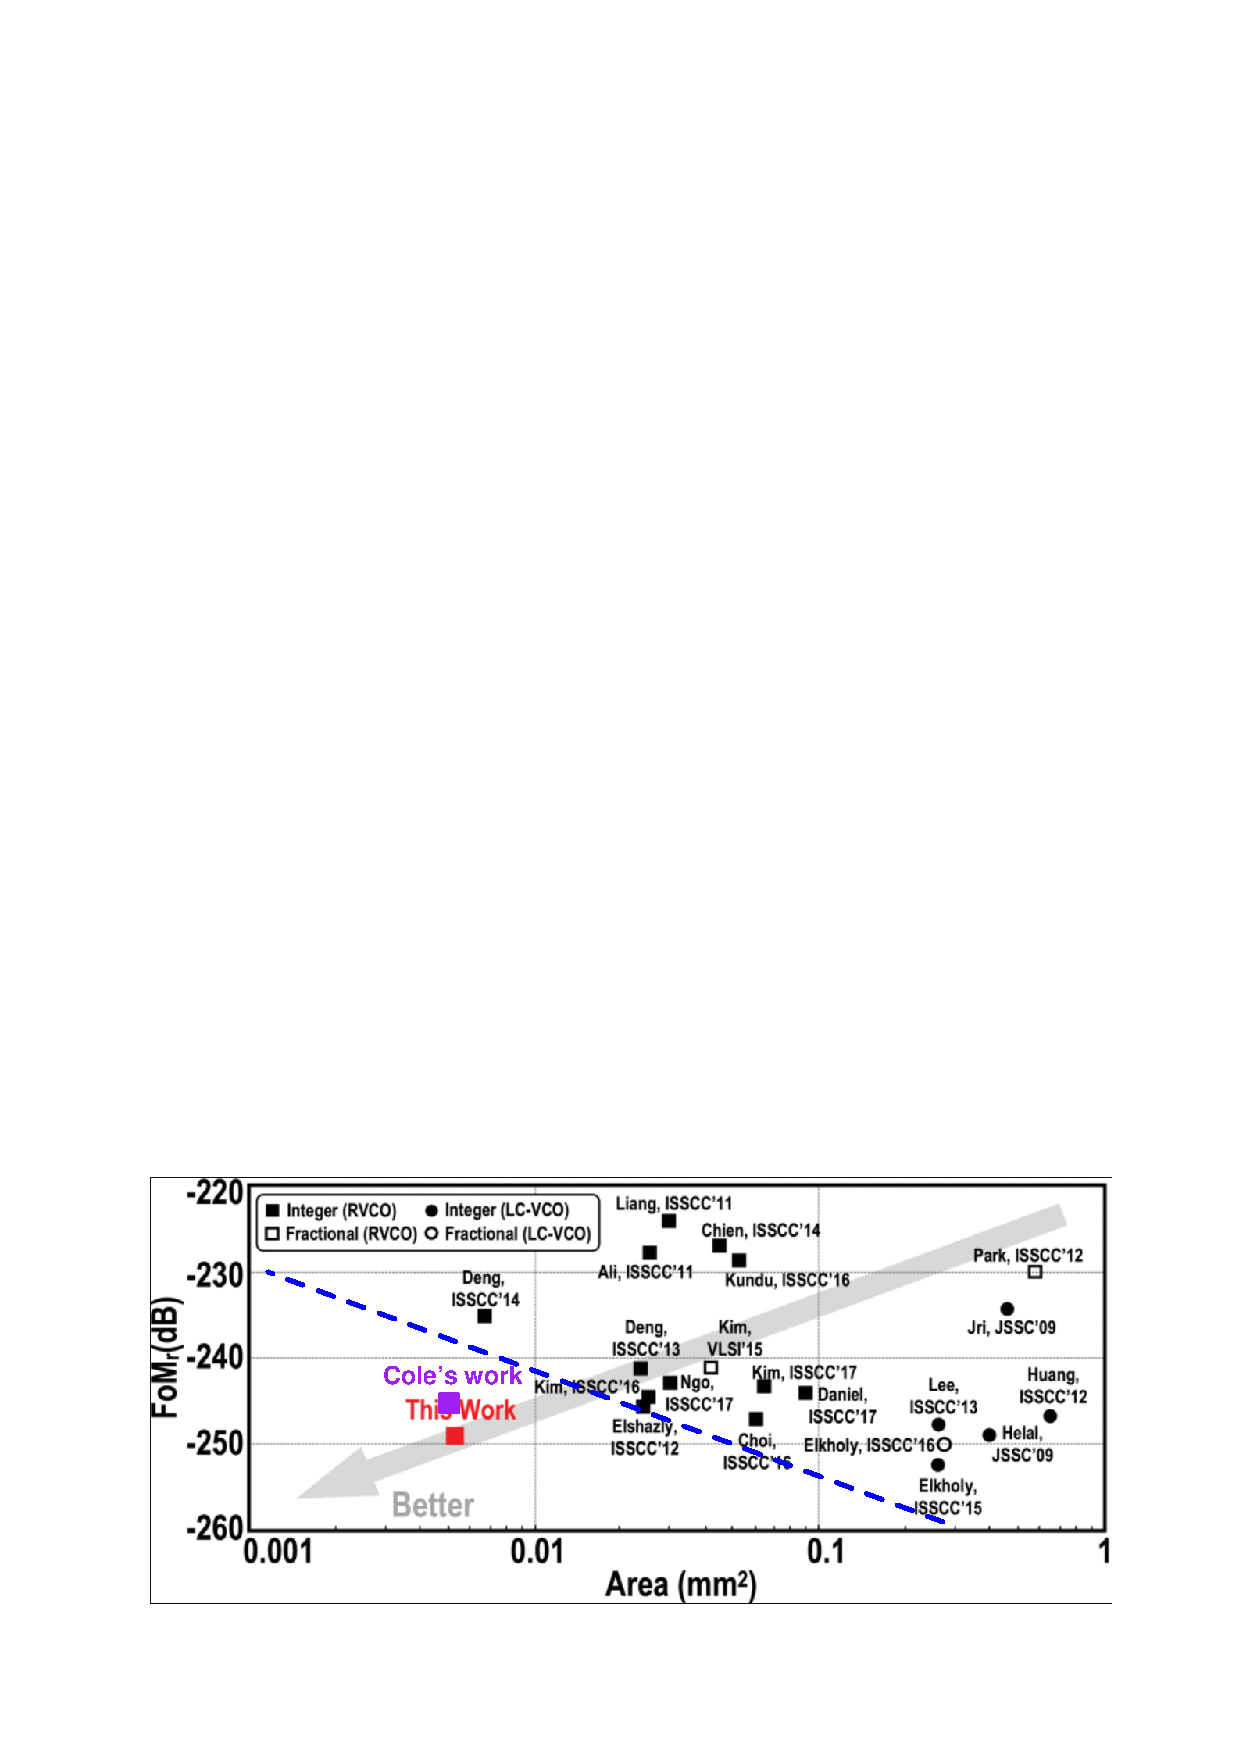
\includegraphics[width=1\textwidth, angle=0]{fom_area_state_art2.pdf}
	\end{minipage}
	\begin{minipage}{6cm}
			\tiny	
			\begin{itemize}[itemsep=4pt,label=\protect---]
				\item Figure from 2019 JSSC paper [2] on a MDLL. Area is 0.0056 mm$^2$ in 28nm technology.
				\item FOM$_r$ here is with normalization to a 200 MHz reference oscillator.
				\item This work uses higher power (1.45 mW), and higher reference (200 MHz), which perhaps explains better FOM.
			\end{itemize} 	
	\end{minipage}
	\end{block}
	\scriptsize
	\vspace{-0.3em}
	{\color{red}\textbf{Verdict:}} \textbf{Competitive in area with state of art (not revolutionary though).}
\end{frame}


\begin{frame}
	\frametitle{New loop filter.}
	\begin{block}{PI-only with changeable filter coefficients.}
		\begin{minipage}{6cm}
			\vspace{1em}
			\tiny

			% \vspace{100em}
			\begin{itemize}[itemsep=4pt,label=\protect---]
				\item Original architecture with 2 feedforward/2 feedback filter coefficients becomes large (ca. 60 $\mu$m x 60 $\mu$m).
				\begin{itemize}[itemsep=4pt,label=\protect$\bullet$]
						\item Implemented fixed pole at zero, and one each of tunable pole/zeros.
						\item With N bit word size, requires 4x NxN array multiplier.
				\end{itemize}
				\item {\color{red}\textbf{Solution:}} reduce to only two feedforward programmable filter coefficients. \textbf{This is a classical PI-controller}.
				\begin{itemize}[itemsep=4pt,label=\protect$\bullet$]
						\item Stability is straightforward, PLL dynamics simpler to model.
						\item Uncompensated zero results in inherent peaking of phase noise spectrum.
				\end{itemize}
				\item \textbf{Also implemented:} On-the-fly changeable filter coefficients to allow for gear switching of the PLL.
			\end{itemize}

			% \vspace{-3em}
		\end{minipage}%
		% \hspace{-0.5cm}
		\begin{minipage}{6cm}
			\begin{figure}[htb!]
			        \centering
			        \includegraphics[width=0.8\textwidth, angle=0]{new_lf}
			    % \caption{Approximate model for ring oscillator inverter delay cell.}
			\end{figure}
		\end{minipage}%

	\end{block}	
\end{frame}

\begin{frame}
	\frametitle{New loop filter.}
	\begin{block}{PI-only with changeable filter coefficients.}
		\begin{minipage}{6cm}
			\vspace{1em}
			\tiny

			% \vspace{100em}
			\begin{itemize}[itemsep=4pt,label=\protect---]
				\item Current filter optimization yields the following minimum resolution requirements:

		\begin{table}[h!]
			\centering
			\def\arraystretch{1.5}		
			\setlength\arrayrulewidth{0.75pt}
			\setlength{\tabcolsep}{1em} % for the horizontal padding
			\begin{tabular}{|c|c|c|c|c|}
				\hline 
				\rule[-1ex]{0pt}{2.5ex} \cellcolor{gray!40}\textbf{Mode} & \cellcolor{gray!40}\textbf{Sign} & \cellcolor{gray!40}\textbf{Integer}& \cellcolor{gray!40}\textbf{Fractional}& \cellcolor{gray!40}\textbf{Sum}\\ 
				\hline 
				\rule[-1ex]{0pt}{2.5ex} \textbf{Counter}  & 1 & 4 & 5 & 10\\ 
				\hline 
				\rule[-1ex]{0pt}{2.5ex} \textbf{BBPD}  & 1 & 4 & 11 & 16\\ 
				\hline 
			\end{tabular} 
			% \caption{Assigned specifications for branch line hybrid design.}
			% \label{asgn_specs}
		\end{table}  
				\item Selection of the input word size xin has been made to equal the counter resolution (8 bit). Accounting for a sign bit this equates to 7 integer bits.
				\item \textbf{Also implemented:} On-the-fly changeable decimal location to allow for gear switching of the PLL.
			\end{itemize}

			% \vspace{-3em}
		\end{minipage}%
		% \hspace{-0.5cm}
		\begin{minipage}{6cm}
			\begin{figure}[htb!]
			        \centering
			        \includegraphics[width=0.5\textwidth, angle=0]{lf_pin_plan}
			    % \caption{Approximate model for ring oscillator inverter delay cell.}
			\end{figure}
		\end{minipage}%

	\end{block}	
\end{frame}



\begin{frame}
	\frametitle{New loop filter.}
	\begin{block}{New split architecture.}
		\begin{minipage}{4cm}
			\vspace{1em}
			\tiny

			% \vspace{100em}
			\begin{itemize}[itemsep=4pt,label=\protect---]
				\item Now use split datapath for counter and BBPD modes.
				\item Reducing to only two feed forward coefficients allows for removal multipliers for BBPD use.
				\begin{itemize}[itemsep=4pt,label=\protect$\bullet$]
						\item Now implemented with muxes.
						\item Lower power/complexity, can use larger word for filter coefficients (24 bit) with little penalty, ie. adder complexity is $\mathcal{O}(n\log n)$, vs $\mathcal{O}(n^2)$ for multipliers.
				\end{itemize} 
			\end{itemize}

			% \vspace{-3em}
		\end{minipage}%
		% \hspace{-0.5cm}
		\begin{minipage}{8cm}
			\begin{figure}[htb!]
			        \centering
			        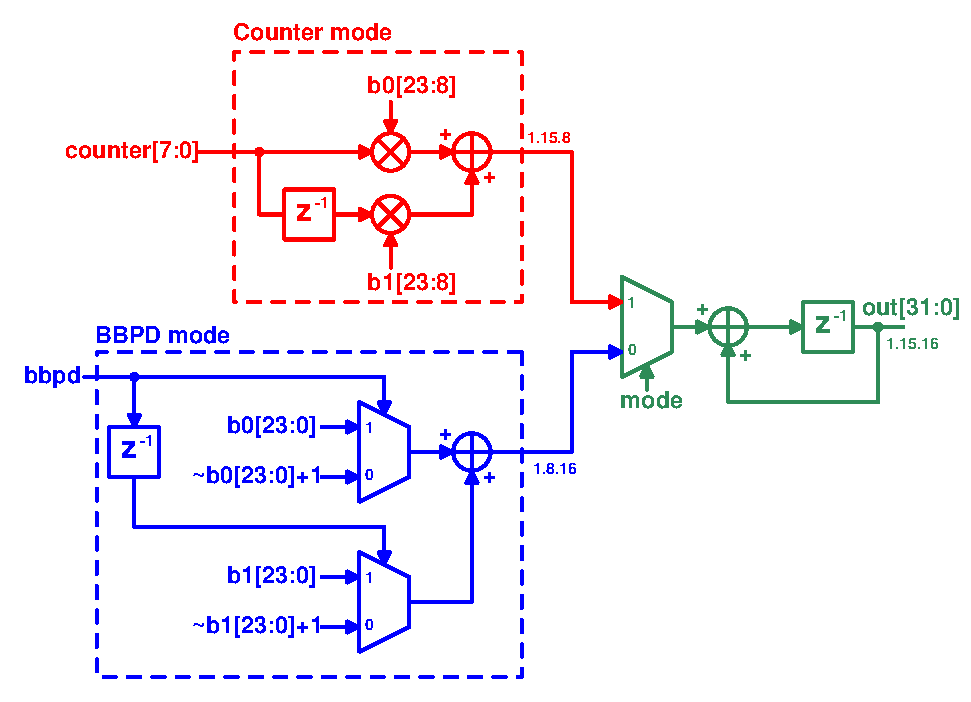
\includegraphics[width=0.8\textwidth, angle=0]{mux_datapath}
			    % \caption{Approximate model for ring oscillator inverter delay cell.}
			\end{figure}
		\end{minipage}%

	\end{block}	
\end{frame}





\begin{frame}
	\frametitle{BBPD-PLL resolution jitter}
	\begin{block}{Resolution/phase quantization effects}
		\begin{figure}
			\includegraphics[width=0.8\textwidth, angle=0]{simplified_bbpll}
		\end{figure}
		\begin{itemize}[itemsep=4pt,label=\protect---]
			\tiny
			\item Output of BBPD is quantized $\pm$ 1. With PI loop filter architecture, there are only 4 possible values that the output {\color{teal}\textbf{w}} can increment by: $\lfloor b_0+b_1 \rfloor$, $\lfloor b_0-b_1 \rfloor$, $\lfloor -b_0+b_1 \rfloor$, $\lfloor -b_0-b_1 \rfloor$.
			\item In steady state, with the BBPD outputting a worst case sequence of +1/-1/+1/-1... , the output will toggle betwwen $\lfloor b_0-b_1 \rfloor$ and $\lfloor -b_0+b_1 \rfloor$.
			\begin{itemize}[itemsep=4pt,label=\protect$\bullet$]
				\item Current optimization yields $b_0$ = 8.899856, $b_1$ = -8.301153 
				\item Thus output {\color{teal}\textbf{w}} will increment by +17, -18, +17, -18 ...
				\item Essentially output will make large-ish jumps in frequency every reference cycle
			\end{itemize}
		\end{itemize}
		\tiny
	\end{block}	
\end{frame}


\begin{frame}
	\frametitle{BBPD-PLL resolution jitter}
	\begin{block}{Worst case estimate (for spurs)}
	\begin{figure}[htb!]
	    \centering
	    \begin{subfigure}{0.5\textwidth}
	        \centering
	        \includegraphics[width=0.8\textwidth, angle=0]{bbpd_resolution_phase_walk}
	    \end{subfigure}%
	    \begin{subfigure}{0.5\textwidth}
	        \centering
	        \center\includegraphics[width=0.8\textwidth, angle=0]{spurs_dco}
	    \end{subfigure}
	    % \caption{Approximate model for ring oscillator inverter delay cell.}
	\end{figure}
		\begin{itemize}[itemsep=4pt,label=\protect---]
			\tiny
			\item Worst case input sequence results in square wave frequency modulation, which in the phase domain creates a cyclostationary triangle wave with period $f_{ref}$/2. This creates \textbf{SPURS} at $f_{ref}$/2.
			\item In general, $f_{ref}$ $>>$ $K_{DCO}|b_0-b_1|$ (frequency deviation), so spurs are not generated at the deviation frequencies.
			\item With 1 LSB deviation per ref. cycle, a -62 dBc spur (SSB) is expected $f_{ref}$/2.
			\begin{itemize}[itemsep=4pt,label=\protect$\bullet$]
			\item Under my current $b_0$, $b_1$, this spur will be -37 dBc.
		\end{itemize}
		\end{itemize}
		\tiny
	\end{block}	
\end{frame}


\begin{frame}
	\frametitle{BBPD-PLL resolution jitter}
	\begin{block}{Total phase noise estimate from resolution jitter.}
			\tiny

			% \vspace{100em}
			\begin{itemize}[itemsep=4pt,label=\protect---]
				\item \textbf{Cyclostationary (+1, -1, +1, -1, ...):}
				\begin{itemize}[itemsep=4pt,label=\protect$\bullet$]
					\item Under my system parameters, the total phase noise power from resolution effects is -34 dBc, essentially all of which is in the first spur at $f_{ref}/2$.
					\begin{equation}
						\Delta \Phi  = \frac{2\pi|b_0-b_1|K_{DCO}}{f_{ref}}
					\end{equation}
					\begin{equation}
						\sigma_{\Phi rj}  = \frac{\pi|b_0-b_1|K_{DCO}}{\sqrt{3}f_{ref}}
					\end{equation}
				\end{itemize}
			\item \textbf{General note:} the phase noise from this source must $<<$ than target SNR for PLL application. Can use these relations to find limits for maximum $K_{DCO}$ before resolution jitter is dominant.			\end{itemize}


	\end{block}	
\end{frame}


\begin{frame}
	\frametitle{BBPD-PLL resolution jitter}
	\begin{block}{Total phase noise estimate from resolution jitter.}
			\tiny

			% \vspace{100em}
			\begin{itemize}[itemsep=4pt,label=\protect---]

				\item \textbf{Average case:}
				\begin{itemize}[itemsep=4pt,label=\protect$\bullet$]
					\item All transitions equally likely out of BBPD.
					\item Under my system parameters, the total phase noise power from resolution effects is -29.4 dBc (simulated).
					\item Phase noise is bimodal. The total RMS phase noise power is approximately equal to the absolute value of the distribution means.
					\begin{equation}
						\mu = \pm\frac{\pi|b_0-b_1|K_{DCO}}{f_{ref}}, \hspace{2em}\sigma_{\Phi rj} \approx |\mu|
					\end{equation}
				\end{itemize}
			\end{itemize}
	\vspace{-3em}
	\begin{figure}[htb!]
	    \centering
	    \begin{subfigure}{0.5\textwidth}
	        \centering
	        \includegraphics[width=0.8\textwidth, angle=0]{bbpd_rw}
	    \end{subfigure}%
	    \begin{subfigure}{0.5\textwidth}
	        \centering
	        \center\includegraphics[width=0.8\textwidth, angle=0]{bbpd_rw_hist}
	    \end{subfigure}
	    % \caption{Approximate model for ring oscillator inverter delay cell.}
	\end{figure}

	\end{block}	
\end{frame}



\begin{frame}
	\frametitle{BBPD Gain.}
	\begin{block}{Additional nonlinearity to an already nonlinear thing...}
		\begin{minipage}{6cm}
			\vspace{1em}
			\tiny

			% \vspace{100em}
			\begin{itemize}[itemsep=4pt,label=\protect---]
				\item Found an interesting dissertation on BBPD PLLs [3], which shows that the linearized BBPD gain model I have been using (K$_{BBPD}$ = $2/\sqrt{2\pi}\sigma_{\Phi_n}$) is not totally correct. 
				\begin{itemize}[itemsep=4pt,label=\protect$\bullet$]
						\item Due to BBPF-PLL resolution jitter, varies depending if resolution jitter or if random noise is the dominant component.
				\end{itemize}
				\item Need to account for this in my filter optimization code...
				\item An approximation, with random/uncorrelated noise with $\sigma_{\Phi uc}$, and resolution jitter $\sigma_{\Phi{rj}}$ (based on variable substitution of [3]'s theory):
				\begin{equation}
					K_{BBPD} = \frac{1}{\sqrt{2\pi}\sigma_{\Phi uc}}\left[1+ e^{-\frac{1}{2}\left(\frac{\sigma_{\Phi{rj}}}{\sigma_{\Phi uc}}\right)^2} \right]
				\end{equation}
					\begin{equation}
						\sigma_{\Phi rj} \approx \frac{\pi|b_0-b_1|K_{DCO}}{f_{ref}}
					\end{equation}
				\item Currently, I should be well into the random noise dominated regime.
			\end{itemize}

			% \vspace{-3em}
		\end{minipage}%
		% \hspace{-0.5cm}
		\begin{minipage}{6cm}
			\begin{figure}[htb!]
			        \centering
			        \includegraphics[width=1\textwidth, angle=0]{kbbpd}
			    % \caption{Approximate model for ring oscillator inverter delay cell.}
			\end{figure}
		\end{minipage}%

	\end{block}	
\end{frame}



\begin{frame}
	\frametitle{Filter optimization}
	\begin{block}{Need to add}
		\begin{enumerate}[itemsep=4pt,label=\protect\mycirc{\arabic*}]
			\tiny
			\item Modeling of BBPD jitter (extracted from circuit simulation).
			\item Account for noise from limit cycle/phase resolution effects.
			\begin{itemize}[itemsep=4pt,label=---]
				\item Adjust $K_{BBPD}$ accordingly
			\end{itemize}
			\item Aliasing/folding of high frequency phase noise into bandwidth of $f_{ref}$ due to sampled nature
			\begin{itemize}[itemsep=4pt,label=---]
				\item Impossible to avoid...
			\end{itemize}
		\end{enumerate}
		\tiny
		Can maybe get better correlation between filter optimization results and discrete time simulation.
		\begin{figure}
			\includegraphics[width=0.4\textwidth, angle=0]{trans_phase_noise_fast}
		\end{figure}
	\end{block}	
\end{frame}







\begin{frame}
	\frametitle{Synthesis/place and route}
	\begin{block}{Loop filter layout.}
	\tiny
	\begin{itemize}[itemsep=4pt,label=\protect---]
		\item First iteration at loop filter layout... still need to extract the circuit/LVS etc...
	\end{itemize}
	\vspace{-1em}
	\begin{figure}[htb!]
	        \centering
	        \includegraphics[width=0.5\textwidth, angle=0]{lf_layout}
	    % \caption{Approximate model for ring oscillator inverter delay cell.}
	\end{figure}

	\end{block}	
\end{frame}






% #############################################################################
% Loop Dynamics (continuous)
% #############################################################################

% \begin{frame}
% 	\frametitle{Loop Dynamics}
% 	\begin{block}{Still To Do}
% 		\vspace{-.2em}
% 		\begin{itemize}
% 			\footnotesize
% 			\item Standard approach to used mixed continuous/discrete time mathematical model for DPLL. 
% 			\item Plot of RO phase noise (typical)
% 			\item Automatic analysis of performance (lock detection, residual phase modulation, lock-in/pull-in range).
% 			\item Automatic optimization (using gradient descent) of PLL parameters?
% 			\item Z-domain modeling of loop? Develop (by hand) some ideal transfer funtions for loop.

% 		\end{itemize}    
% 	\end{block}
% \end{frame}

% #############################################################################
% Architecture - block diagram
% #############################################################################


\begin{frame}
	\frametitle{Architecture}
	\begin{block}{Block Diagram}
	\center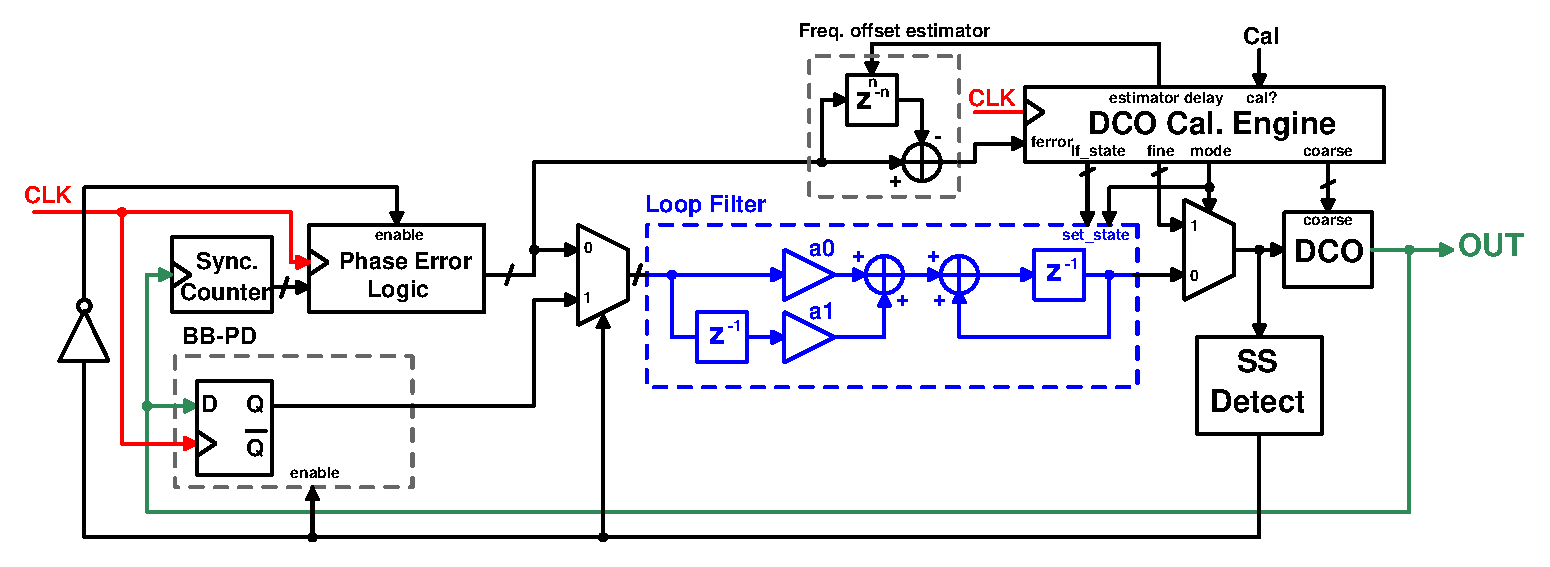
\includegraphics[width=0.8\textwidth, angle=0]{pll_master_arch_28feb2020}

	\end{block}
		\begin{block}{Power Targets {\color{red}(revised)}}
		\scriptsize
		{\color{red}\textbf{(Divider not necessary)}}
		\vspace{-1em}
		\begin{table}[htb!]
			\tiny
			\centering
			\def\arraystretch{1.5}		
			\setlength\arrayrulewidth{0.75pt}
			\setlength{\tabcolsep}{1em} % for the horizontal padding
			\begin{tabular}{|c|c|c|c|c|}
				\hline 
				\rule[-1ex]{0pt}{2.5ex} \cellcolor{gray!40}\textbf{DCO} & \cellcolor{gray!40}\textbf{Phase detector} & \cellcolor{gray!40}\textbf{Digital (LF)}& \cellcolor{gray!40}\textbf{Other} & \cellcolor{gray!40}\textbf{SUM} \\ 
				\hline 
				\rule[-1ex]{0pt}{2.5ex} 50 $\mu$W& 10 $\mu$W &  10 $\mu$W  & \textbf{0} {\color{red}\st{$\leq$ 5}} $ \mu$W & $\leq$ \textbf{70} {\color{red}\st{100}} $\mu$W\\ 
				\hline 
			\end{tabular} 
			% \caption{Assigned specifications for branch line hybrid design.}
			% \label{asgn_specs}
		\end{table}   
	\end{block}

\end{frame}

% #############################################################################
% Specification
% #############################################################################

\begin{frame}
	\frametitle{Specification\color{black}}
	\begin{block}{System Performance Targets}
		\tiny
		\begin{table}[h!]
			\centering
			\def\arraystretch{1.5}		
			\setlength\arrayrulewidth{0.75pt}
			\setlength{\tabcolsep}{1em} % for the horizontal padding
			\begin{tabular}{|l|r|l|l|}
				\hline 
				\rule[-1ex]{0pt}{2.5ex} \cellcolor{gray!40}\textbf{Parameter} & \cellcolor{gray!40}\textbf{Value} & \cellcolor{gray!40}\textbf{Unit }& \cellcolor{gray!40}\textbf{Notes}\\ 
				\hline 
				\rule[-1ex]{0pt}{2.5ex} \textbf{Frequency}  & 2.4-2.4835 & GHz & 2.4G ISM Band\\ 
				\hline 
				\rule[-1ex]{0pt}{2.5ex} \textbf{Ref. frequency} & 16 & MHz & Yields 6 channels \\ 
				\hline 
				\rule[-1ex]{0pt}{2.5ex} \textbf{Power} & $\leq$ \textbf{70} {\color{red}\st{75}} $\mu$W  &$\mu$W & Minimize!\\ 
				\hline 
				\rule[-1ex]{0pt}{2.5ex} \textbf{FSK BER} & $\leq$ 1e-2  & & GFSK\textbf{*} with $f_{dev}$=$\pm$250 KHz\\ 
				\hline 
				\rule[-1ex]{0pt}{2.5ex} \textbf{CNR} & $>$ 20 & dBc&Yields  \textbf{-235} dB FOM$_{jitter}$ ideally \\ 
				\hline 
				\rule[-1ex]{0pt}{2.5ex} \textbf{Initial Lock Time} & $\leq$ 10 & $\mu$s & Upon cold start \\ 
				\hline 
				\rule[-1ex]{0pt}{2.5ex} \textbf{Re-lock Time} & $\leq$ 5 & $\mu$s & Coming out of standby, $f_{error} <$ \textbf{1 MHz} \\ 
				\hline 
				\rule[-1ex]{0pt}{2.5ex} \textbf{Lock $\Delta f$ tolerance} & $100$ & kHz& \\ 
				\hline 
				\rule[-1ex]{0pt}{2.5ex} \textbf{FOM}$_{\textnormal{jitter}}$ & $\leq$ -230 & dB & \textbf{For state of art in size/power} \\ 
				\hline 
				\rule[-1ex]{0pt}{2.5ex} \textbf{Area} & $<$ 0.01  & mm$^2$ & \\ 
				\hline 
			\end{tabular} 
			% \caption{Assigned specifications for branch line hybrid design.}
			% \label{asgn_specs}
		\end{table}   
		\textbf{*} Using BT=0.3, 1 MSymbols/s, 4 demodulated symbols averaged per bit to yield 250 kbps.
	\end{block}    
\end{frame}



\begin{frame}
	\frametitle{Specification\color{black}}
	\begin{block}{Component-level specs}
		\scriptsize
	\begin{table}[h!]
		\centering
		\tiny
		\def\arraystretch{1.5}		
		\setlength\arrayrulewidth{0.75pt}
		\setlength{\tabcolsep}{1em} % for the horizontal padding
		\begin{tabular}{|l|r|l|}
			\hline 
			\rule[-1ex]{0pt}{2.5ex} \cellcolor{gray!40}\textbf{Parameter} & \cellcolor{gray!40}\textbf{Value} & \cellcolor{gray!40}\textbf{Unit }\\ 
			\hline 
			\rule[-1ex]{0pt}{2.5ex} \textbf{Counter range}  & 256 steps & coverage of 150-155 \\ 
			\hline 
			\rule[-1ex]{0pt}{2.5ex} \textbf{Divider ratio} & 150-155  & (For non-counter based)\\ 
			\hline 
			\rule[-1ex]{0pt}{2.5ex} {\color{red}\st{\textbf{TDC resolution}}} &{\color{red}\st{$\geq$ 155}}  & {\color{red}\st{steps/reference cycle}}\\ 
			\hline 
			\rule[-1ex]{0pt}{2.5ex} \textbf{DCO gain $K_{DCO}$} & $10^4$ & Hz/LSB \\ 
			\hline 
			\rule[-1ex]{0pt}{2.5ex} \textbf{DCO tuning range} & 10 & MHz \\ 
			\hline 
			\rule[-1ex]{0pt}{2.5ex} \textbf{DCO DAC resolution} & 10 & bit \\ 
			\hline 
			\rule[-1ex]{0pt}{2.5ex} \textbf{DCO Phase noise} &$<$ -80 & dBc/Hz @ $\Delta f=10^6$ Hz, $f_c$ = 2.448 GHz \\ 
			\hline 
			\rule[-1ex]{0pt}{2.5ex} \textbf{DCO Power} & $\leq$ 50 & $\mu$W \\ 
			\hline 
			\rule[-1ex]{0pt}{2.5ex} \textbf{Digital filter word resolution} & $\leq$ 16 & bits (power grows as $\mathcal{O}(n^2)$) \\ 
			\hline 
			\rule[-1ex]{0pt}{2.5ex} \textbf{BB-PD jitter} & $\leq$ 12 & ps$_{\textnormal{rms}}$ \\ 
			\hline 
		\end{tabular} 
		% \caption{Assigned specifications for branch line hybrid design.}
		% \label{asgn_specs}
		\label{design_specs}
	\end{table}   
	\end{block}    
\end{frame}

% #############################################################################
% Timeline
% #############################################################################

\begin{frame}
	\frametitle{Time plan (pt. 1)}
	\begin{table}[htb!]
		\tiny
		\centering
		\vspace{-1em}
		\def\arraystretch{1.5}		
		\setlength\arrayrulewidth{0.75pt}
		\setlength{\tabcolsep}{1em} % for the horizontal padding
		\begin{tabular}{|c|l|l|l|}
			\hline 
			\rule[-1ex]{0pt}{2.5ex}\cellcolor{gray!40}\textbf{Week \#} & \cellcolor{gray!40}\textbf{Dates} &\cellcolor{gray!40}\textbf{Tasks} & \cellcolor{gray!40}\textbf{Outcomes}\\ 
			\hline 
			% \rule[-1ex]{0pt}{2.5ex} \cellcolor{green!20}\textbf{3}&\cellcolor{green!20}13.1 - 19.1 &\cellcolor{green!20}Review PLL Design &\cellcolor{green!20}Refreshed Knowledge\\ 
			% \hline 
			\rule[-1ex]{0pt}{2.5ex}\cellcolor{red!40}\textbf{4}&\cellcolor{red!40}20.1 - 26.1 &\cellcolor{red!40}Finalize high level modeling &\cellcolor{red!40}Component level specification\\ 
			\hline 
			\rule[-1ex]{0pt}{2.5ex}\textbf{5}\cellcolor{red!40}&\cellcolor{red!40}27.1 - 2.2 &\cellcolor{red!40}Establish test bench in Virtuoso &\cellcolor{red!40}With ideal PLL implementation\\ 
			\hline 
			\rule[-1ex]{0pt}{2.5ex}\cellcolor{red!40}\textbf{6}&\cellcolor{red!40}3.2 - 9.2&\cellcolor{red!40}Schem. design: phase detector &\cellcolor{red!40}TDC - flash and counter based \\ 
			\hline 
			\rule[-1ex]{0pt}{2.5ex}\cellcolor{red!40}\textbf{7}&\cellcolor{red!40}10.2 - 16.2&\cellcolor{red!40}Schem. design: phase detector &\cellcolor{red!40}Bang-bang phase detector\\ 
			\hline 
			\rule[-1ex]{0pt}{2.5ex}\cellcolor{red!40}\textbf{8}&\cellcolor{red!40}17.2 - 23.2&\cellcolor{red!40}RTL, synthesis, place\&route &\cellcolor{red!40}Digital loop filter\\ 
			\hline 
			\rule[-1ex]{0pt}{2.5ex}\cellcolor{green!40}\textbf{9}&\cellcolor{green!40}24.2 - 1.3&\cellcolor{green!40}RTL, synthesis, place\&\cellcolor{green!40}route & \cellcolor{green!40}Digital loop filter\\ 
			\hline 
			\rule[-1ex]{0pt}{2.5ex}\textbf{10}&2.3 - 8.3& Schem. design: oscillator & Ring DCO\\ 
			\hline 
			\rule[-1ex]{0pt}{2.5ex}\textbf{11}&9.3 - 15.3& Layout: oscillator & \\ 
			\hline 
			\rule[-1ex]{0pt}{2.5ex}\textbf{12}&16.3 - 22.3& CDAC  & Schem+layout\\ 
			\hline 
			\rule[-1ex]{0pt}{2.5ex}\textbf{13}&23.3 - 29.3& Calibration& RTL/schem. for calibration\\ 
			\hline 
			\rule[-1ex]{0pt}{2.5ex}\textbf{14}& 30.3 - 5.4 &  Flex week - schem. design & Finalize schematic level design\\ 
			\hline 
			\rule[-1ex]{0pt}{2.5ex}\textbf{15}& 6.4 - 12.4& {\color{red}\textbf{Easter}} & - \\ 
			\hline 
			\rule[-1ex]{0pt}{2.5ex}\textbf{16}& 13.4 - 19.4& Layout & Phase detector\\ 
			\hline 
			\rule[-1ex]{0pt}{2.5ex}\textbf{17}& 20.4 - 26.4& Layout & Oscillator\\ 
			\hline 
		\end{tabular}
		\begin{flushleft}\textbf{Legend:} \colorbox{red!20}{\textbf{Done}} \colorbox{green!20}{\textbf{Current}}  \colorbox{blue!20}{\textbf{Revised}}
		% *I will write the report simultaneously with the work.
		\end{flushleft}
		% \caption{Assigned specifications for branch line hybrid design.}
		% \label{asgn_specs}
	\end{table}   
\end{frame}

\begin{frame}
	\frametitle{Time plan (pt. 2)}
	\begin{table}[htb!]
		\tiny
		\centering
		\vspace{-1em}
		\def\arraystretch{1.5}		
		\setlength\arrayrulewidth{0.75pt}
		\setlength{\tabcolsep}{1em} % for the horizontal padding
		\begin{tabular}{|c|l|l|l|}
			\hline 
			\rule[-1ex]{0pt}{2.5ex}\cellcolor{gray!40}\textbf{Week \#} & \cellcolor{gray!40}\textbf{Dates} &\cellcolor{gray!40}\textbf{Tasks} & \cellcolor{gray!40}\textbf{Outcomes}\\ 
			\hline 
			\rule[-1ex]{0pt}{2.5ex}\textbf{18}& 27.4 - 3.5 & Layout & Divider/calibration\\ 
			\hline 
			\rule[-1ex]{0pt}{2.5ex}\textbf{19}& 4.5 - 10.5 & Layout & Finalization/system integration\\ 
			\hline 
			\rule[-1ex]{0pt}{2.5ex}\textbf{20}& 11.5 - 17.5 & Flex week (layout) OR yield improvement & Depending on progress\\ 
			\hline 
			\rule[-1ex]{0pt}{2.5ex}\textbf{21}& 18.5 - 24.5& {\color{blue}\textbf{Report writing}} & \\ 
			\hline 
			\rule[-1ex]{0pt}{2.5ex}\textbf{22}& 25.5 - 31.5& {\color{blue}\textbf{Report writing}} & \\ 
			\hline 
			\rule[-1ex]{0pt}{2.5ex}\textbf{23}& 1.6 - 7.6& {\color{blue}\textbf{Report writing}} & {\color{red}\textbf{Deadline 8.6}}\\ 
			\hline 
		\end{tabular}
		\begin{flushleft}\textbf{Legend:} \colorbox{red!20}{\textbf{Done}} \colorbox{green!20}{\textbf{Current}}  \colorbox{blue!20}{\textbf{Revised}}
		% *I will write the report simultaneously with the work.
		\end{flushleft}
		% \caption{Assigned specifications for branch line hybrid design.}
		% \label{asgn_specs}
	\end{table}   
\end{frame}


% #############################################################################
% project phases
% #############################################################################

% ############################################################################b#
% References
% #############################################################################


\begin{frame}
	\frametitle{References}
		\scriptsize
		[1] Liu, B., Li, Z., Fu, X., Shirane, A., Kurosu, H., Nakane, Y., Masaki, S., Okada, K., Zhang, Y., Qiu, J., Huang, H., Sun, Z., Xu, D., Zhang, H., Wang, Y. and Pang, J. (2020). A Fully-Synthesizable Fractional-N Injection-Locked PLL for Digital Clocking with Triangle/Sawtooth Spread-Spectrum Modulation Capability in 5 nm CMOS. IEEE Solid-State Circuits Letters, pp.1-1.\par
		% [1]  Liu, H., Shirane, A., Okada, K., Sun, Z., Huang, H., Deng, W., Siriburanon, T., Pang, J., Wang, Y., Wu, R. and Someya, T. (2019). A 265-$\mu$ W Fractional-${N}$ Digital PLL With Seamless Automatic Switching Sub-Sampling/Sampling Feedback Path and Duty-Cycled Frequency-Locked Loop in 65-nm CMOS. IEEE Journal of Solid-State Circuits, 54(12), pp.3478-3492.
		\vspace{0.5em}
		[2] Yang, S., Yin, J., Mak, P. and Martins, R. (2019). A 0.0056-mm2 -249-dB-FoM All-Digital MDLL Using a Block-Sharing Offset-Free Frequency-Tracking Loop and Dual Multiplexed-Ring VCOs. IEEE Journal of Solid-State Circuits, 54(1), pp.88-98.\par
		\vspace{0.5em}
		[3] N. Da Dalt, "Linearized analysis of a digital bang-bang PLL and its validity limits applied to jitter transfer and jitter generation", IEEE Trans. Circuits Syst. I, vol. 55, pp. 3663-3675, Dec. 2008.

		% [1]  H. Xu and A. A. Abidi, “Design Methodology for Phase-Locked Loops Using Binary (Bang-Bang) Phase Detectors,” IEEE Transactions on Circuits and Systems I: Regular Papers, vol. 64, no. 7, pp. 1637–1650, Jul. 2017.\par
		% \vspace{0.5em}
		% [2] F. Gardner, “Charge-Pump Phase-Lock Loops,” IEEE Transactions on Communications, vol. 28, no. 11, pp. 1849–1858, Nov. 1980, doi: 10.1109/tcom.1980.1094619.\par
		% \vspace{0.5em}
		% [3] Liu, B., Li, Z., Fu, X., Shirane, A., Kurosu, H., Nakane, Y., Masaki, S., Okada, K., Zhang, Y., Qiu, J., Huang, H., Sun, Z., Xu, D., Zhang, H., Wang, Y. and Pang, J. (2020). A Fully-Synthesizable Fractional-N Injection-Locked PLL for Digital Clocking with Triangle/Sawtooth Spread-Spectrum Modulation Capability in 5 nm CMOS. IEEE Solid-State Circuits Letters, pp.1-1.
	% Navid et al. 2005
\end{frame}


\end{document}
